\documentclass[a4paper,hidelinks,14pt]{extarticle}

\usepackage[T2A]{fontenc}
\usepackage[utf8]{inputenc}
\usepackage[russian]{babel}
\usepackage{cmap}

\usepackage{xcolor}

\usepackage{helvet}
\usepackage{pscyr}


\usepackage{multicol}

% \usepackage{amssymb,amsfonts,amsmath,mathtext}
% \usepackage{cite,enumerate,float}

\graphicspath{{images/}}      % Подключаемые пакеты
%%% Макет страницы %%%
\geometry{a4paper,top=20mm,bottom=27mm,left=30mm,right=15mm}
\setstretch{1.15}

%%% Язык текста %%%
\selectlanguage{russian}

%%% Кодировки и шрифты %%%
\renewcommand{\rmdefault}{ftm} % Включаем Times New Roman

%%% Выравнивание и переносы %%%
\sloppy				% Избавляемся от переполнений
\clubpenalty=10000		% Запрещаем разрыв страницы после первой строки абзаца
\widowpenalty=10000		% Запрещаем разрыв страницы после последней строки абзаца
\interfootnotelinepenalty=10000 % Запрет разрывов сносок

%%% Нумерация страниц %%%
\fancypagestyle{empty}{%
\fancyhf{} % clear all header and footer fields
\renewcommand{\headrulewidth}{0pt}
\renewcommand{\footrulewidth}{0pt}
\setlength{\headheight}{5mm} 
}

\fancypagestyle{plain}{%
\fancyhf{} % clear all header and footer fields
\fancyfoot[R]{\thepage} 
\renewcommand{\headrulewidth}{0pt}
\renewcommand{\footrulewidth}{0pt}
\setlength{\headheight}{5mm}
}

\pagestyle{plain}

%%% Библиография %%%

\makeatletter
\bibliographystyle{ugost2003s} % Оформляем библиографию в соответствии с ГОСТ 7.1 2003

\let\oldthebibliography=\thebibliography
\let\endoldthebibliography=\endthebibliography
\renewenvironment{thebibliography}[1]{
  \begin{oldthebibliography}{#1}
    \setlength{\parskip}{0mm}
    \setlength{\itemsep}{0mm}
}
{
\end{oldthebibliography}
}

%%% Изображения %%%
\graphicspath{{images/}} % Пути к изображениям

%%% Содержание %%%
\renewcommand{\cfttoctitlefont}{\hfil \large\bfseries}

\setlength{\cftparskip}{0mm}
\setlength{\cftbeforesecskip}{0mm}
\setlength{\cftaftertoctitleskip}{14pt}

\renewcommand{\cftsecaftersnumb}{\:}
\renewcommand{\cftsecfont}{}   
\renewcommand{\cftsecpagefont}{\normalsize}
\renewcommand{\cftsecleader}{\cftdotfill{\cftdotsep}}
\setlength{\cftsecindent}{0mm}
\setlength{\cftsecnumwidth}{3mm}

\setlength{\cftsubsecindent}{4mm}
\setlength{\cftsubsecnumwidth}{8mm}

%%% Требования ЕСКД/СТП %%%

%%% Размеры заголовков
\newcommand{\sectionbreak}{\clearpage}

\titleformat{\section}{\large\bfseries}{\thesection}{\wordsep}{}
\titlespacing*{\section}{12mm}{14pt}{14pt}

\titleformat{name=\section,numberless}{\large\bfseries\filcenter}{}{0mm}{}
\titlespacing*{name=\section,numberless}{0mm}{14pt}{14pt}

\titleformat{name=\subsection}{\normalsize\bfseries}{\thesubsection}{\wordsep}{}
\titlespacing*{\subsection}{12mm}{14pt}{14pt}

\titleformat{name=\subsection,numberless}{\normalsize\bfseries}{}{0mm}{}
\titlespacing*{name=\subsection,numberless}{0mm}{14pt}{14pt}

%%% Нумерация параграфов

\counterwithout{paragraph}{subsubsection}
\counterwithin{paragraph}{subsection}
\renewcommand{\theparagraph}{\thesubsection.\arabic{paragraph}}
\setcounter{secnumdepth}{4}

\titleformat{name=\paragraph}[runin]{\normalsize\bfseries}{\theparagraph}{\wordsep}{}
\titlespacing*{\paragraph}{12mm}{14pt}{\wordsep}

%%% Размеры текста формул %%%

\DeclareMathSizes{12}{12}{6}{4}

%%% Расстояние между формулами

\AtBeginDocument{%
  \setlength\abovedisplayskip{14pt}%
  \setlength\belowdisplayskip{14pt}%
  \setlength\abovedisplayshortskip{14pt}%
  \setlength\belowdisplayshortskip{14pt}%
}

%%% Оформление текста

\setlength{\parskip}{0pt}
\setlength{\parindent}{12mm}

%%% Расстояние между плавающими элементами

\setlength{\floatsep}{14pt}     % between top floats
\setlength{\textfloatsep}{14pt} % between top/bottom floats and text
\setlength{\intextsep}{14pt}    % between text and float
\setlength{\dbltextfloatsep}{14pt}
\setlength{\dblfloatsep}{14pt}

 % костыль для того, чтобы убрать расстояние от картинки до текста
\setlength{\abovecaptionskip}{0pt}
\setlength{\belowcaptionskip}{0pt}
           
%%% Оформление списков
\AddEnumerateCounter{\asbuk}{\@asbuk}{\cyrm}

\setlist{nosep,listparindent=\parindent}
\setlist[1]{itemindent=18.5mm,leftmargin=0mm,itemsep=0mm,topsep=0mm,parsep=0mm}             
\setlist[itemize,1]{label=$-$}
\setlist[enumerate,1]{label=\arabic*)}

\setlist[2]{itemindent=20.5mm,leftmargin=0mm,itemsep=0mm,topsep=0mm,parsep=0mm}             

% Определяем новый стиль для списков,
% на которые есть ссылки в тексте
\newlist{reflist}{enumerate*}{1}
\setlist*[reflist,1]{%
  label=\asbuk*),
}

\setlist*[reflist,2]{%
  label=\arabic*),
}

%% Нумерация плавающих элементов

\counterwithin{figure}{section}
\counterwithin{table}{section}

\makeatletter
\AtBeginDocument{%
\renewcommand{\thetable}{\thesection.\arabic{table}}
\renewcommand{\thelstlisting}{\thesection.\arabic{lstlisting}}
\renewcommand{\thefigure}{\thesection.\arabic{figure}}
\let\c@lstlisting\c@figure}
\makeatother 

%% Подписи плавающих элементов

\captionsetup[figure]{
  labelsep=endash,
  justification=centering,
  singlelinecheck=false,
  position=bottom,
  skip=14pt}

\captionsetup[table]{
  labelsep=endash,
  justification=raggedright,
  singlelinecheck=false,
  position=top,
  skip=0mm}

\captionsetup[lstlisting]{
  labelsep=endash
}

\lstset{
basicstyle=\scriptsize\ttfamily,
numberstyle=\scriptsize\ttfamily,
keywordstyle=\bfseries,
commentstyle=\itshape,
numbers=left,
stepnumber=1,
frame=single,
resetmargins=true,
xleftmargin=7mm,
xrightmargin=2mm,
captionpos=b,
keepspaces=true,
breaklines=true,
aboveskip=22pt,
belowskip=10pt,
abovecaptionskip=16pt}

\renewcommand{\arraystretch}{1.5}

%%% Настройка размеров вертикальных отступов

\renewcommand{\smallskip}{\vspace{6pt}}
\renewcommand{\bigskip}{\vspace{14pt}}
	      % Пользовательские стили
                       
\begin{document}          
%%% Переопределение именований %%%
\renewcommand{\abstractname}{Аннотация}
\renewcommand{\alsoname}{см. также}
\renewcommand{\appendixname}{Приложение}
\renewcommand{\bibname}{Литература}
\renewcommand{\ccname}{исх.}
\renewcommand{\chaptername}{Глава}
\renewcommand{\contentsname}{СОДЕРЖАНИЕ}
\renewcommand{\enclname}{вкл.}
\renewcommand{\figurename}{Рисунок}
\renewcommand{\lstlistingname}{Рисунок}
\renewcommand{\headtoname}{вх.}
\renewcommand{\indexname}{Предметный указатель}
\renewcommand{\listfigurename}{Список рисунков}
\renewcommand{\listtablename}{Список таблиц}
\renewcommand{\pagename}{Стр.}
\renewcommand{\partname}{Часть}
\renewcommand{\seename}{см.}
\renewcommand{\tablename}{Таблица}

\renewcommand{\refname}{СПИСОК ИСПОЛЬЗОВАННЫХ ИСТОЧНИКОВ}
	      % Переопределение именований
                          
\thispagestyle{empty}
\setlength{\parindent}{0ex} % set paragraph indenting to zero

\begin{center}
  Министерство образования Республики Беларусь \\
  \vspace{0.5ex}
  Учреждение образования \\
  БЕЛОРУССКИЙ ГОСУДАРСТВЕННЫЙ УНИВЕРСИТЕТ \\
  ИНФОРМАТИКИ И РАДИОЭЛЕКТРОНИКИ \\
  \vspace{0.5ex}
  Факультет информационных технологий и управления \\
  \vspace{0.5ex}
  Кафедра информационных технологий автоматизированных систем
\end{center}

\vspace{50mm}

\begin{center}
  Отчет по лабораторной работе № 4 \\
  <<Модульное программирование на языке Ассемблер>>
\end{center}

\vspace{60mm}

\begin{minipage}{.55\linewidth}
    Выполнил студент группы 120602

    \smallskip

    Проверил
\end{minipage}
\hfill
\begin{minipage}{.4\linewidth}
  \begin{flushright}
    Будный Р. И. \_\_\_\_\_\_\_\_\_\_

    \smallskip

    Гончаревич А. Л. \_\_\_\_\_\_\_\_\_\_
  \end{flushright}
\end{minipage}

\vspace{50mm}
\begin{center}
  Минск 2014
\end{center}

\setlength{\parindent}{1.25cm} % reset paragraph indenting

\newpage
	      % Титульный лист

\setcounter{page}{5}

\tableofcontents
     % Содержание
\section*{ВВЕДЕНИЕ}
\addcontentsline{toc}{section}{Введение}

Планирование промышленного производства является важной составляющей 
экономических расчётов, имеющих целью организацию высокоэффективного 
и прибыльного производства.
Планирование позволяет на ранних этапах предусмотреть все возможные затраты и
риски, которые могут возникнуть при организации производства,
оценить примерную цену изделия,
рассчитать основные технико-экономические показатели функционирования предприятия.

Целью данной курсовой работы является расчёт календарно-плановых нормативов
и технико-экономическое обоснование производства изделия для предприятия.
Объектом производства является кронштейн, применяемый при выпуске
радиоэлектронной аппаратуры. 
Расчёт будет выполняться в соответствии с методикой расчёта и 
исходными данными, приведенными в методических пособиях~\cite{opiup_1,opiup_2}.
        % Введение
\section[Обоснование типа производства и вида поточной линии]{
  ОБОСНОВАНИЕ ТИПА ПРОИЗВОДСТВА И ВИДА \\
  ПОТОЧНОЙ ЛИНИИ
}
\label{sec:choice}

\subsection[
Краткое описание объекта производства и технологического \\
процесса
]{
  Краткое описание объекта производства и 
  технологического процесса
}

Объектом производства является кронштейн,
применяющийся при изготовлении радиоэлектронных изделий.
Характеристика кронштейна как объекта производства приведена
в таблице~\ref{tbl:piece_description}.

\begin{table} [h!]
  \caption{
    Краткая характеристика объекта производства
  }\label{tbl:piece_description}
  {\small
    \begin{tabular}{| m{2.7cm} | m{1.7cm} | m{2.1cm} | m{1.9cm} | m{1.4cm} | m{1.8cm} | m{1.8cm} |}
      \hline
      Наименование детали & Вид заготовки & Материал, марка
      & Вес заготовки, кг & Чистый вес детали, кг
      & Оптовая цена 1 кг металла, у.~е. & Оптовая цена 1 кг отходов, у.~е. \\
      \hline
      Кронштейн & Прокат & Ст. А12-ТВ
      & 0{,}20 & 0{,}12 
      & 0{,}16 & 0{,}05 \\
      \hline
    \end{tabular}
  }
\end{table}

Месячная программа выпуска кронштейна составляет 5000 шт.,
режим работы двухсменный, количество рабочих дней --- 23,
процент потерь рабочего времени --- 3\%, продолжительность смены --- 8 ч.
Цены и нормы расхода материала для технологического 
процесса изготовления кронштейна приведены в таблице~\ref{tbl:tech_process}.

{\small
\begin{longtable}{| m{2.5cm} | c | m{2.5cm} | c | c | c | c | c | c |}
  \caption{Технологический процесс изготовления детали}\label{tbl:tech_process} \\
      \hline
      \rotatebox[origin=c]{90}{\hspace{0.01mm}
      \parbox{3.5cm}{Наименование \\ операции}}
      & \rotatebox[origin=c]{90}{\parbox{3.5cm}{Разряд работы}}
      & \rotatebox[origin=c]{90}{\parbox{3.5cm}{Наименование оборудования}}
      & \rotatebox[origin=c]{90}{\parbox{3.5cm}{Модель оборудования или марка}}
      & \rotatebox[origin=c]{90}{\parbox{3.5cm}{Габариты  оборудования}}
      & \rotatebox[origin=c]{90}{\parbox{3.5cm}{Мощность, кВт}}
      & \rotatebox[origin=c]{90}{\parbox{3.5cm}{Оптовая цена, у.~е.}}
      & \rotatebox[origin=c]{90}{\parbox{3.5cm}{Коэффициент выполнения норм}} 
      & \rotatebox[origin=c]{90}{\parbox{3.5cm}{
        Норма времени \\ ( \( t_{\text{шт}} \) ), мин}} \\
      \hline
      \centering 1 & 2 & \centering 3 & 4 & 5 & 6 & 7 & 8 & 9 \\
      \hline
      \endfirsthead 

      \multicolumn{8}{l}{\normalsize Продолжение таблицы \thetable{}} \\
      \hline
      \centering 1 & 2 & \centering 3 & 4 & 5 & 6 & 7 & 8 & 9 \\
      \hline
      \endhead

      1. Фрезерная & 3 & Универсаль- ный фрезерный станок 
      & 6Р82Ш & 2470x1250 & 8{,}0
      & 2400 & 1{,}1 & 6{,}4 \\
      \hline
      2. Шлифова- льная & 4 & Плоскошли- фовальный станок
      & 3Б71м1 & 2600x1550 & 7{,}0
      & 3800 & 1{,}1 & 8{,}2 \\
      \hline
      3. Слесарная & 3 & Верстак
      & НДР-1064 & 1200x700 & --
      & 360 & 1{,}1 & 9{,}2 \\
      \hline
      4. Токарная & 4 & Токарно-винторезный станок
      & 1А616П & 2135x1225 & 10{,}0
      & 4425 & 1{,}1 & 4{,}0 \\
      \hline
      5. Фрезерная & 4 & Универса- льный фрезерный станок 
      & 6Р82Ш & 2470x1950 & 8{,}0
      & 2400 & 1{,}1 & 7{,}6 \\
      \hline
      6. Слесарная & 3 & Верстак
      & НДР-1064 & 1200x700 & --
      & 360 & 1{,}13 & 5{,}0 \\
      \hline
      7. Сверлиль- ная & 3 & Настольно-сверлильный станок
      & НС-12А & 710x360 & 3{,}5
      & 630 & 1{,}1 & 6{,}8 \\
      \hline
      8. Токарная & 4 & Токарно-винторезный станок
      & 1А616П & 2135x1225 & 10{,}0
      & 4425 & 1{,}1 & 7{,}0 \\
      \hline
\end{longtable}
}

\subsection[
Выбор и обоснование типа производства и вида поточной линии \\
(участка)
]{
  Выбор и обоснование типа производства и
  вида поточной линии (участка)
}

Вычислим коэффициент специализации \( K_{\text{сп}} \), 
такт выпуска изделий \( r_{\text{н.п.}}\) и
коэффициент массовости \( K_\text{м} \):
\begin{align*}
K_{\text{сп}} &= \dfrac{m}{C_{\text{пр}}} = \dfrac{8}{5} = 1{,}6, \\
r_{\text{н.п.}} &= \dfrac{60 F_{\text{э}}}{N_{\text{з}}} = 
  \frac{60 F_{\text{н}} F_{\text{п.о}}}{N_{\text{з}}} =
  \dfrac{60 \cdot 23 \cdot 8 \cdot 2 \cdot 0{,}95}{5000} =
  4{,}20 \: \text{(мин/шт.)}, \\
K_{\text{м}} &=
\dfrac{\sum^m_{i=1} t_{\text{шт}_{i}}}{m \cdot r_{\text{н.п.}}} = 
\dfrac{
  \frac{6{,}4}{1{,}1} + \frac{8{,}2}{1{,}1} + \frac{9{,}2}{1{,}1} + 
  \frac{4{,}0}{1{,}1} + \frac{7{,}6}{1{,}1} + \frac{5{,}0}{1{,}13} +
  \frac{6{,}8}{1{,}1} + \frac{7{,}0}{1{,}1}
}{
  8 \cdot 4{,}2
} = 1{,}46.
\end{align*}

Поскольку \( K_{\text{сп}} < 2 \) и \( K_{\text{м}} > 1 \),
следовательно, тип производства массовый.
Кроме этого, нормы времени выполнения операций не кратны такту, 
поэтому целесообразна организация поточного производства на основе
однопредметной прерывно-поточной линии.       % Обоснование типа производства и вида поточной линии
\section[%
Расчет календарно-плановых нормативов и построение стандарт-плана]{
РАСЧЕТ КАЛЕНДАРНО-ПЛАНОВЫХ \\
НОРМАТИВОВ И ПОСТРОЕНИЕ \\
СТАНДАРТ-ПЛАНА
}
\label{sec:kpn}

Основной состав календарно-плановых нормативов ОНПЛ:
\begin{itemize}
  \item такт или ритм потока;
  \item количество рабочих мест по операциям и по всей поточной линии;
  \item скорость движения конвейера;
  \item период конвейера и система адресования;
  \item величина заделов;
  \item длительность производственного цикла;
  \item стандарт-план ОНПЛ;
  \item темп поточной линии;
  \item мощность, потребляемая конвейером.
\end{itemize}

Такта выпуска изделий был рассчитан в подразделе~\ref{subsec:choice},
$r_{\text{н.п.}}~=~0{,}72$~мин/шт.

\subsection{Определение количества рабочих мест по операциям и по всей поточной линии}
\label{subsec:number_of_employees_calculation}

Для определения количества рабочих мест по операциям необходимо произвести
синхронизацию технологического процесса. Синхронизацию технологического
процесса сведём в таблицу~\ref{tbl:technology_synchronization}.

Рассчитанное количество рабочих мест по всей поточной линии в
таблице~\ref{tbl:technology_synchronization} позволяет произвести выбор
и обосновать тип производства и вид поточной линии (подраздел~\ref{subsec:choice}).

\newpage

\begin{table} [h!]
  \caption{%
    Синхронизация технологического процесса
  }\label{tbl:technology_synchronization}
  {\small
    \begin{tabular}{| m{0.4cm} | m{2.1cm} | m{1.3cm} | m{2.1cm} | m{0.8cm} | m{2.1cm} | m{2.1cm} | m{2.1cm} |}
      \hline
      \rotatebox[origin=c]{90}{\hspace{2mm}\parbox{3.5cm}{№ операции}} &
      \rotatebox[origin=c]{90}{\hspace{2mm}\parbox{3.5cm}{\vspace{6mm}Норма штучного \newline времени, $t_{\text{шт.}}$, мин}} &
      \rotatebox[origin=c]{90}{\hspace{2mm}\parbox{3.5cm}{Коэффициент выполнения \newline норм, $K_{\text{в}}$ }} &
      \rotatebox[origin=c]{90}{\hspace{2mm}\parbox{3.5cm}{\vspace{3mm}Норма штучного \newline времени с учётом \newline $K_{\text{в}}$, $t_{\text{шт.}}^{'}$, мин}} &
      \rotatebox[origin=c]{90}{\hspace{2mm}\parbox{3.5cm}{Такт линии, \newline $r_{\text{п.л.}}$, мин/шт. }} &
      \rotatebox[origin=c]{90}{\hspace{2mm}\parbox{3.5cm}{\vspace{8mm}Расчётное $C_p$ }} &
      \rotatebox[origin=c]{90}{\hspace{2mm}\parbox{3.5cm}{\vspace{8mm}Принятое $C_{\text{пр}}$ }} &
      \rotatebox[origin=c]{90}{\hspace{2mm}\parbox{3.5cm}{Коэффициент загрузки \newline рабочих мест, \newline оборудования, $K_{\text{з}}$ }} \\
      \hline

      1 & 1,42 & 1,00 & 1,42 & 0,72 & 1,96 & 2 & 0,98 \\ \hline
      2 & 0,70 & 1,00 & 0,70 & 0,72 & 0,97 & 1 & 0,97 \\ \hline
      3 & 0,68 & 1,00 & 0,68 & 0,72 & 0,94 & 1 & 0,94 \\ \hline
      4 & 0,70 & 1,00 & 0,70 & 0,72 & 0,97 & 1 & 0,97 \\ \hline
      5 & 2,11 & 1,00 & 2,11 & 0,72 & 2,92 & 3 & 0,97 \\ \hline
      6 & 0,72 & 1,00 & 0,72 & 0,72 & 1,00 & 1 & 1,00 \\ \hline
      7 & 0,67 & 1,00 & 0,67 & 0,72 & 0,93 & 1 & 0,93 \\ \hline
      8 & 2,10 & 1,00 & 2,10 & 0,72 & 2,90 & 3 & 0,97 \\ \hline
      9 & 0,70 & 1,00 & 0,70 & 0,72 & 0,97 & 1 & 0,97 \\ \hline
      \multicolumn{5}{| l |}{Итого:} & 13,54 & 14 & \\ \hline

    \end{tabular}
  }
\end{table}

\subsection{Определение периода конвейера и системы адресования}

Период конвейера определяется как наименьшее общее кратное количества рабочих
мест на операциях.
\begin{align*}
  \text{П} = \text{НОК(2,1,1,1,3,1,1,3,1)} = 6.
\end{align*}

В таблице~\ref{tbl:conveyor_marker} изобразим разметку конвейера.
\begin{table} [h!]
  \caption{
    Разметка конвейера
  }\label{tbl:conveyor_marker}
  {\small
    \begin{tabular}{ c | c | c | c | c | c | c | c | c | c }
      \hline
      1 & 2 & 3 & 4 & 5 & 6 & 1 & 2 & 3 & ... \\ \hline
      \multicolumn{6}{| c |}{П} & $l_{\text{пр}}$

    \end{tabular}
  }
\end{table}

Далее произведём закрепление номеров периода за каждым рабочим местом, в
соответствии с которым каждый рабочий должен брать и класть предметы труда
на ленту конвейера. Порядок закрепления номеров за рабочими местами приведен
в таблице~\ref{tbl:numbers_fixation}.

\newpage

\begin{table} [h!]
  \caption{
    Порядок закрепления номеров за рабочими местами
  }\label{tbl:numbers_fixation}
  {\small
    \begin{tabular}{| m{2.0cm} | m{2.0cm} | m{2.0cm} | m{4.1cm} | m{4.1cm} |}
      \hline
      № операции &
      Число рабочих мест &
      Номер рабочего места &
      Число закреплённых номеров за \newline рабочим местом &
      Последовательность закреплённых номеров за \newline рабочим местом \\
      \hline

      \multirow{2}{*}{1} & \multirow{2}{*}{2} & 1 & 3 & 1, 3, 5 \\
                                            \cline{3-5}
                                            & & 2 & 3 & 2, 4, 6 \\
      \hline

      2 & 1 & 3 & 6 & 1, 2, 3, 4, 5, 6 \\ \hline
      3 & 1 & 4 & 6 & 1, 2, 3, 4, 5, 6 \\ \hline
      4 & 1 & 5 & 6 & 1, 2, 3, 4, 5, 6 \\ \hline

      \multirow{3}{*}{5} & \multirow{3}{*}{3} & 6 & 2 & 1, 4 \\
                                            \cline{3-5}
                                            & & 7 & 2 & 2, 5 \\
                                            \cline{3-5}
                                            & & 8 & 2 & 3, 6 \\
      \hline

      6 & 1 & 9  & 6 & 1, 2, 3, 4, 5, 6 \\ \hline
      7 & 1 & 10 & 6 & 1, 2, 3, 4, 5, 6 \\ \hline

      \multirow{3}{*}{8} & \multirow{3}{*}{3} & 11 & 2 & 1, 4 \\
                                            \cline{3-5}
                                            & & 12 & 2 & 2, 5 \\
                                            \cline{3-5}
                                            & & 13 & 2 & 3, 6 \\
      \hline

      9 & 1 & 14 & 6 & 1, 2, 3, 4, 5, 6 \\ \hline

    \end{tabular}
  }
\end{table}


\subsection{Определение длины ленты конвейера}

Если шаг конвейера $l_{\text{пр}}$ на всех операциях принять равным $1{,}1$ м, то
рабочая длина конвейера вычисляется следующим образом:
\begin{align*}
  L_{p} = C_{\text{пр}} \cdot l_{\text{пр}} = 14 \cdot 1{,}1 = 15{,}4~(\text{м}).
\end{align*}

Полная длина ленты конвейера $L_n$ должна быть несколько больше
двойной рабочей длины конвейера и должна быть согласована с условием
распределения, определяемом по формуле:
\begin{align*}
  L_n &= 2 \cdot L_p + \pi \cdot \text{Д} \hspace{5mm} \le \hspace{5mm} K \cdot \text{П} \cdot l_{\text{пр}}, \\
  K   &= \dfrac{L_n}{\text{П} \cdot l_{\text{пр}} }
\end{align*}

При диаметре натяжного и приводного барабанов $ \text{Д} = 0{,}4$ (м) получаем:
\begin{align}
\label{eq:temp}
  L_n &= 2 \cdot 15{,}4 + \pi \cdot 0{,}4 = 32{,}06~(\text{м}) \hspace{5mm} \le \hspace{5mm} 5 \cdot 6 \cdot 1{,}1 = 33~(\text{м}), \\
  K   &= \dfrac{ 32{,}06 }{ 6 \cdot 1{,}1 } = 4{,}86 \approx 5. \nonumber
\end{align}

Видно, что условие~\ref{eq:temp} выполняется, значит шаг конвейера $l_{\text{пр}}$
не нуждается в корректировке.


\subsection{Определение скорости ленты конвейера}

Скорость ленты конвейера определяется по формуле:
\begin{align*}
  v = \dfrac{ l_{\text{пр}} }{ r_{\text{н.п.}} } = \dfrac{1{,}1}{0{,}72} = 1{,}52~ (\text{м/мин}).
\end{align*}


\subsection{Определение мощности, потребляемой конвейером}

Определим производительность $\rho$ поточной линии по формуле:
\begin{align*}
  \rho = \dfrac{1}{r_{\text{н.п.}}} \cdot 60 = \dfrac{1}{0{,}72} \cdot 60 = 82{,}9~(\text{шт./ч}).
\end{align*}

Часовая производительность конвейера в единицах массы при среднем весе
единицы продукции $Q = 0{,}18 $~(кг):
\begin{align*}
  q_r = \rho \cdot Q = 82{,}9 \cdot 0{,}18 = 14{,}93~(\text{кг/ч}).
\end{align*}

Мощность, потребляемая конвейером определяется по формуле при весе ленты~(цепи)
конвейера $Q = 6$~кг/пог.м:
\begin{align*}
  W &= 1{,}2 \cdot \Big[ \dfrac{ 0{,}16 \cdot L_n \cdot v \cdot Q_k }{ 36 } + \dfrac{ 0{,}16 \cdot L_n \cdot q_r }{ 270 } \Big] , \\
  W &= 1{,}2 \cdot \Big[ \dfrac{ 0{,}16 \cdot 32{,}06 \cdot 1{,}52 \cdot 6 }{ 36 } + \dfrac{ 0{,}16 \cdot 32{,}06 \cdot 14{,}93 }{ 270 } \Big] = 1{,}90~(\text{л.с.}), \\
  P_{\text{уст.}} &= 0{,}736 \cdot W = 0{,}736 \cdot 1{,}90 = 1{,}4~(\text{кВт}).
\end{align*}


\subsection{Расчёт заделов}

На производстве с однопредметной непрерывно-поточной линией создаются заделы
трёх видов: технологический, транспортный и страховой (резервный).

Технологический задел --- количество изделий, которое в каждый момент времени
находится в процессе обработки на рабочих местах. При поштучной передаче изделий
он соответствует числу рабочих мест, таким образом:
\begin{align*}
  Z_{\text{техн}} = C_{\text{пр}} = 14~(\text{шт.}).
\end{align*}

Транспортный задел --- количество изделий, которое в каждый момент времени
находится на конвейере в процессе транспортировки. Для поштучной передаче
изделий определяется по формуле:
\begin{align*}
  Z_{\text{тр}} = C_{\text{пр}} - 1 = 14 - 1 = 13~(\text{шт.}).
\end{align*}

Резервный задел создаётся на линиях с наиболее ответственных или же нестабильных
по времени выполнения операциях, а также на контрольных пунктах. Определяется
по формуле:
\begin{align*}
  Z_{\text{рез}} = \dfrac{t_{\text{рез}}}{r_{\text{н.п.}}}.
\end{align*}

В расчётах $ t_{\text{рез}} $ принимают как $ 4 - 5\% $ штук изделий от сменного
задания. В итоге имеем:
\begin{align*}
  N_{\text{см}} &= \dfrac{30597}{23 \cdot 2} = 665~(\text{шт.}), \\
  Z_{\text{рез}} &= \dfrac{t_{\text{рез}}}{r_{\text{н.п.}}} = \dfrac{665 \cdot 0{,}05}{0{,}72} = 46~(\text{шт.}).
\end{align*}

Общая величина задела определяется как сумма технологического, транспортного и
резервного заделов:
\begin{align*}
  Z_{\text{общ}} = Z_{\text{техн}} + Z_{\text{тр}} + Z_{\text{рез}} = 14 + 13 + 46 = 73~(\text{шт.}).
\end{align*}


\subsection{Расчёт величины незавершенного производства}

Величина незавершенного производства без учёта затрат времени в предыдущем цехе
определяется по формуле:
\begin{align*}
  H_{\text{в}} = Z_{\text{общ}} \cdot \dfrac{\sum\limits_{i=1}^m t_i}{2} = 73 \cdot \dfrac{9{,}8}{2 \cdot 60} = 5{,}96~(\text{нормо-ч}).
\end{align*}

Величина незавершенного производства в денежном выражении при цеховой себестоимости
изделия, находящегося в заделе $C_z = 0{,}85 \cdot C_{\text{ц}}$,
где $ C_{\text{ц}} $ -- цеховая себестоимость изделия законченной обработки:

\textbf{CHECK $C_{\text{ц}}$ HERE}.
\begin{align*}
  H_{\text{з}} = Z_{\text{общ}} \cdot C_z = Z_{\text{общ}} \cdot 0{,}85 \cdot C_{\text{ц}} = 73 \cdot 0{,}85 \cdot = ~(\text{у.е.}).
\end{align*}

\subsection{Расчёт длительности производственного цикла и построение стандарт-плана}

Длительность производственного цикла определяется графическим (на основе
стандарт-плана) и аналитическим способом.

\textbf{РАСЧЁТ АНАЛИТИЧЕСКИМ СПОСОБОМ}

Стандарт-план работы участка расположен в приложении~\ref{sec:appendix_a}.
          % Расчет календарно-плановых нормативов и
                          % построение стандарт-плана
\section[
Расчет производственной площади и планировка участка]{
РАСЧЕТ ПРОИЗВОДСТВЕННОЙ ПЛОЩАДИ И \\
ПЛАНИРОВКА УЧАСТКА
}
\label{sec:placement}

\subsection{Планировка производственного участка}

Поточная линия имеет П-образную форму во избежание перекрещивающихся и
обратных потоков материалов и предметов труда.
Планировка производственного участка расположена в приложении Б.
Сырьё поступает на универсальный фрезерный станок, 
расположенный в  левом нижнем углу схемы, 
проходит через указанные в таблице~\ref{tbl:tech_process} стадии
технологического процесса и завершается на контрольном столе,
который обозначен в правом нижнем углу плана.

\subsection{Расчет производственной площади участка}

Расчет производственной площади участка, занимаемой технологическим оборудованием
(рабочими местами) и транспортными средствами, 
приведен в таблице~\ref{tbl:prod_placement}.
Расчет общей площади участка приведен в таблице~\ref{tbl:common_placement}.

По результатам расчетов, общую площадь цеха примем равной
180 \( \text{м}^2 \) (18x10 м).

\begin{table} [h!]
  \caption{
    Расчет производственной площади участка
  }\label{tbl:prod_placement}
    \begin{tabular}{
      | m{4.3cm} | c | c | c | c | c |}
      \hline
      \parbox{4.3cm}{\centering Наименование \\ оборудования}
      & \rotatebox[origin=c]{90}{\parbox{4.5cm}{Модель (марка)}}
      & \rotatebox[origin=c]{90}{\parbox{4.5cm}{Габаритные размеры, мм}}
      & \rotatebox[origin=c]{90}{
        \parbox{4.5cm}{
            Количество единиц \\ оборудования (\( C_{\text{пр}} \))
          }
        }
      & \rotatebox[origin=c]{90}{
        \parbox{4.5cm}{
            Коэффициент дополнительной площади (\( K_{\text{дп}} \))
          }
        }
      & \rotatebox[origin=c]{90}{
        \parbox{4.5cm}{
            Производственная \\ площадь участка \\ (\( S \)), \( \text{м}^2 \)
          }
        } \\
      \hline

      Универсальный фрезерный станок & 6Р82Ш & 2470x1250 & 4 & 3{,}5 & 43{,}23 \\
      \hline

      Плоско- шлифовальный станок & 3Б71м1 & 2600x1550 & 2 & 3{,}0 & 24{,}18 \\
      \hline 

      Верстак & НДР-1064 & 1200x700 & 3 & 4{,}0 & 10{,}08 \\
      \hline 

      Токарно-винторезный станок & 1А616П & 2135x1225 & 3 & 3{,}5 & 27{,}46 \\
      \hline 

      Настольно-сверлильный станок & НС12А & 710x360 & 2 & 4{,}0 & 2{,}04 \\
      \hline 

      Контрольный стол & & 1200x700 & 1 & 4{,}0 & 3{,}36 \\
      \hline 

      Электрокар & ЭП201 
      & \parbox{3cm}{
        \smallskip
        \centering Трасса \\ 12000x1500
        \smallskip
      } & 1 & 1{,}0 & 18{,}00 \\
      \hline 

      \raggedleft \textbf{Итого} & & & \textbf{16} & & \textbf{128{,}35} \\
      \hline 
    \end{tabular}
\end{table}

\begin{table} [h!]
  \caption{
    Расчет общей площади участка
  }\label{tbl:common_placement}
    \begin{tabular}{| m{5.8cm} | m{5.75cm} | c |}
      \hline
      \parbox{5.8cm}{
        \smallskip
        \centering Вид  площади
        \smallskip
      }
      & \parbox{5.75cm}{
          \smallskip
          \centering Источник \\ или методика расчета
          \smallskip
      }
      & Площадь (\( S \)), \( \text{м}^2 \) \\
      \hline

      1. Производственная \newline площадь 
      & \centering См.~таблицу~\ref{tbl:prod_placement}
      & 128{,}35 \\
      \hline

      2. Вспомогательная \newline площадь 
      & \centering Принимаем 40\% \newline от производственной
      & 51{,}34 \\
      \hline
      
      \raggedleft \textbf{Итого} & & \textbf{179{,}69} \\
      \hline
    \end{tabular}
\end{table}

\subsection{Обоснование выбора типа здания}

Продукция, производимая на данном промышленном предприятии,
отличается небольшой массой и относительно небольшим количеством средств труда.
В связи с этим целесообразно размещать такое производство в многоэтажном здании;
допустимо размещение указанного цеха на любом этаже.

Помещение цеха имеет форму прямоугольника, габаритные размеры 18x10 м, 
площадь 180 \( \text{м}^2 \).
Ширина пролета принята равной \( L = 9 \: \text{м} \),
т.~е. имеются два пролета, образованные железобетонными колоннами. 
Шаг колонн равен \( t = 6 \: \text{м} \), с учетом этого в каждом ряду находится
по две колонны.
Таким образом, для поддержания перекрытий цеха следует использовать шесть колонн.
Стены здания выполняются из железобетонных панелей высотой 1{,}2 м и
имеют высоту 3{,}6 м.
    % Расчет производственной площади и планировка участка
\section[%
Расчёт мощности, потребляемой оборудованием и транспортными \\
средствами]{%
  РАСЧЁТ МОЩНОСТИ, ПОТРЕБЛЯЕМОЙ \\
  ОБОРУДОВАНИЕМ И  ТРАНСПОРТНЫМИ \\
  СРЕДСТВАМИ
}
\label{sec:placement}

Расчёт мощности, потребляемой оборудованием и транспортными средствами,
приведен в таблице~\ref{tbl:tech_power}.

\begin{table} [h!]
  \caption{
    Расчёт установленной мощности, потребляемой
    оборудованием и транспортными средствами
  }\label{tbl:tech_power}
    \begin{tabular}{| m{4cm} | m{2cm} | m{2cm} | c | c |}
      \hline
      \multirow{2}{*}{\parbox{4cm}{
          \smallskip
          \centering Наименование оборудования
          \smallskip
        }
      }
      & \multirow{2}{*}{\parbox{2cm}{
            \smallskip
            \centering Модель (марка)
            \smallskip
          }
        }
      & \multirow{2}{*}{\parbox{2cm}{
            \smallskip
            \centering Кол-во единиц
            \smallskip
          }
        }
      & \multicolumn{2}{c|}{Установленная мощность, кВт} \\ \cline{4-5}

      & &
      & \parbox{3cm}{\centering единицы}
      & \parbox{3cm}{\centering принятого} \\
      \hline

      Конвейер & \centering ЭП-201
      & \centering 1 & 0,57 & 0,57 \\
      \hline

      Паяльник & \centering --
      & \centering 1 & 0,05 & 0,05 \\
      \hline

      Установка <<Волна>> & \centering --
      & \centering 3 & 14,00 & 42,00 \\
      \hline

      Испытательный стенд & \centering --
      & \centering 1 & 14,00 & 14,00 \\
      \hline

      \textbf{Итого} & \centering \textbf{--}
      & \centering \textbf{6} & \textbf{--} & \textbf{56{,}62} \\
      \hline
    \end{tabular}
\end{table}
        % Расчет мощности, потребляемой оборудованием и
                          % транспортными средствами
\section[Расчёт стоимости и амортизации основных производственных фондов]{%
  РАСЧЁТ СТОИМОСТИ И АМОРТИЗАЦИИ \\
  ОСНОВНЫХ ПРОИЗВОДСТВЕННЫХ ФОНДОВ
}
\label{sec:amortization}

\subsection[%
Расчёт стоимости здания, занимаемого участком производства]
{Расчёт стоимости здания, занимаемого участком производства}

Расчёт стоимости здания, занимаемого производственным участком,
и амортизационных отчислений приведен в таблице~\ref{tbl:placement_cost}.

\begin{table} [h!]
  \caption{
    Расчёт стоимости здания и амортизационных отчислений
  }\label{tbl:placement_cost}
    \begin{tabular}{| m{6.6cm} | c | c | c | c | c |}
      \hline
      \parbox{6.6cm}{
        \smallskip
        \centering Элементы расчета
        \smallskip
      }
      & \rotatebox[origin=c]{90}{
          \parbox{4.5cm}{
            Стоимость 1 \( \text{м}^2 \) \\ здания, у.~е./\( \text{м}^2 \)
          }
        }
      & \rotatebox[origin=c]{90}{
          \parbox{4.5cm}{
            Площадь, \\ занимаемая \\ зданием, \( \text{м}^2 \)
          }
        }
      & \rotatebox[origin=c]{90}{
          \parbox{4.5cm}{
            Стоимость \\ здания, у.~е.
          }
        }
      & \rotatebox[origin=c]{90}{
          \parbox{4.5cm}{
            Норма амортизации,~\%
          }
        }
      & \rotatebox[origin=c]{90}{
          \parbox{4.5cm}{
            Сумма амортизационных отчислений, у.~е.
          }
        } \\
      \hline

      1. Производственная площадь & 170 & 79,47 & 13~509,9
      & 2{,}7 & 364,8 \\
      \hline

      2. Вспомогательная площадь & 250 & 19,87 & 4~967,5
      & 3{,}1 & 154{,}0 \\
      \hline

      \textbf{Итого} & \textbf{--} & \textbf{99{,}33}
      & \textbf{18~477,4} & \textbf{--} & \textbf{518,8} \\
      \hline
    \end{tabular}
\end{table}

\vspace{-5mm}

\subsection{Расчёт затрат на оборудование и транспортные средства}

Расчёт затрат на оборудование и транспортные средства
приведен в таблице~\ref{tbl:tech_cost}. Величина затрат на упаковку,
транспортировку, монтаж и пусконаладочные работы принята равной 10\%
от цены оборудования.

Расчёт стоимости конвейера производится исходя из его рабочей длинны ($ L_n $),
стоимости одного погонного метра пролётной части (31,77~у.е. для ширины
транспортного средства, равной 400~мм) и стоимости электродвигателя~(принимаем
35\% от стоимости конвейера):
\begin{align*}
  \text{ПС}_{\text{конв}} = (1 + 0{,}35) \cdot 31{,}77 \cdot 32{,}06 = 1~374{,}9~\text{у.е.}.
\end{align*}

\begin{table} [h!]
  \caption{
    Расчёт стоимости транспортного и технологического оборудования
  }\label{tbl:tech_cost}
  {\small
    \begin{tabular}{| m{2.8cm} | c | c | c | c | c | c | c | c |}
      \hline
      \multirow{2}{*}{
        \rotatebox[origin=c]{90}{
          \parbox{6cm}{
            Наименование технологического \\
            оборудования и \\
            транспортных средств
          }
        }
      }
      & \multirow{2}{*}{
          \rotatebox[origin=c]{90}{
            \parbox{6cm}{
              Модель (марка)
            }
          }
        }
      & \multirow{2}{*}{
          \rotatebox[origin=c]{90}{
            \parbox{6cm}{
              Количество единиц оборудова- \\
              ния, транспортных средств, шт.
            }
          }
        }
      & \multicolumn{2}{c|}{Оптовая цена}
      & \multirow{2}{*}{
          \rotatebox[origin=c]{90}{
            \parbox{6cm}{
              Затраты на упаковку, \\
              транспортировку, монтаж, \\
              пуск, наладку, у.~е.
            }
          }
        }
      & \multirow{2}{*}{
          \rotatebox[origin=c]{90}{
            \parbox{6cm}{
              Балансовая (первоначальная) \\
              стоимость техники, у.~е.
            }
          }
        }
      & \multirow{2}{*}{
          \rotatebox[origin=c]{90}{
            \parbox{6cm}{
              Норма амортизации, у.~е.
            }
          }
        }
      & \multirow{2}{*}{
          \rotatebox[origin=c]{90}{
            \parbox{6cm}{
              Сумма амортизационных \\
              отчислений, у.~е.
            }
          }
        } \\ \cline{4-5}

      & &
      & \rotatebox[origin=c]{90}{
          \parbox{5.3cm}{
            единицы, у.~е.
          }
        }
      & \rotatebox[origin=c]{90}{
          \parbox{5.3cm}{
            принятого кол-ва, у.~е.
          }
        }
      & & & & \\
      \hline

      1. Верстак & НДР-1064
      & 14
      & 360 & 5~040 & 504 & 5~544
      & 8,2 & 454,6 \\
      \hline

      2. Конвейер & --
      & 1
      & 1~374,9 & 1~374,9 & 137,5 & 1~512,4
      & 14,8 & 223,8 \\
      \hline

      3. Установка \newline <<Волна>> & --
      & 3
      & 510 & 1~530 & 153 & 1~683
      & 15,7 & 264,2 \\
      \hline

      4. Испытатель- \newline ный стенд & --
      & 1
      & 380 & 380 & 38 & 418
      & 8,1 & 33,9 \\
      \hline

      5. Паяльник & --
      & 1
      & 150 & 150 & 15 & 165
      & 14,3 & 23,6 \\
      \hline

      \textbf{Итого} & \textbf{--}
      & \textbf{20}
      & \textbf{--} & \textbf{8~474,9} & \textbf{847,5} & \textbf{9~322{,}4}
      & \textbf{--} & \textbf{1~000{,}1} \\
      \hline
    \end{tabular}
  }
\end{table}


\subsection{Расчёт затрат на энергетическое оборудование}

Величина затрат на силовое энергетическое оборудование, его монтаж,
упаковку, транспортировку, определяемая исходя из норматива 45 у.е.
на 1 кВт установленной мощности технологического и транспортного
оборудования, составляет:
\begin{equation*}
  \text{ПС}_{\text{э}} = 45 \cdot 56{,}62 = 2~547{,}9~(\text{у.е.}).
\end{equation*}


\subsection{Расчёт затрат на комплект дорогостоящей оснастки, УСПО и \\
инструмента}

Величина затрат на дорогостоящую оснастку, УСПО,
инструмент (первоначальный фонд), принимаемая в размере 10\% от
балансовой стоимости технологического оборудования, составляет:
\begin{equation*}
  \text{ПС}_{\text{ос}} = 0{,}1 \cdot 9~322{,}4 = 932{,}2 ~(\text{у.е.}).
\end{equation*}


\subsection{Расчёт затрат на измерительные и регулирующие приборы}

Величина затрат на измерительные и регулирующие приборы,
принимаемая в размере 1{,}5-2{,}0\% от
оптовой цены оборудования, составляет:
\begin{equation*}
  \text{ПС}_{\text{из}} = 0{,}0175 \cdot 8~474{,}9 = 148{,}3 ~(\text{у.е.}).
\end{equation*}


\subsection{Расчёт затрат на производственный и хозяйственный инвентарь}

Величина затрат на производственный инвентарь,
принимаемая в размере $1{,}5-2{,}0~\%$ от
стоимости технологического оборудования, а также
затрат на хозяйственный инвентарь
(по $15{,}4$~у.е. на одного работающего), составляет:
\begin{equation*}
  \text{ПС}_{\text{ин}} =
  0{,}0175 \cdot 9~322{,}4 + 15{,}4 \cdot \textbf{??} = \textbf{????{,}??} \: (\text{у.~е.}).
\end{equation*}

\subsection{Расчёт стоимости основных производственных фондов и \\
амортизационных отчислений}

Расчёт затрат на оборудование и транспортные средства
приведен в таблице~\ref{tbl:common_cost}.

\begin{table} [h!]
  \caption{
    Расчёт стоимости основных производственных фондов и
    амортизационных отчислений
  }\label{tbl:common_cost}
  {\small
    \begin{tabular}{| m{6.3cm} | c | c | c | c |}
      \hline
        \parbox{6.3cm}{
          \smallskip
          \centering Наименование групп основных производственных фондов
          \smallskip
        }
      & \parbox{1cm}{
          \smallskip
          \centering Усл. \\ обозн.
        }
      & \parbox{2.3cm}{
        \smallskip
          \centering Стоимость производ- ственных фондов, у.~е.
        }
      & \parbox{2.3cm}{
          \centering Норма амортизации, \%
        }
      & \parbox{2.4cm}{
          \centering Сумма аморт. отчислений, у.~е., в мес
        } \\
      \hline

      1. Здание, занимаемое участком
      & \( K_{\text{зд}} \)
      & 18~477,4 & Таблица~\ref{tbl:placement_cost} & 43,23 \\
      \hline

      2. Технологическое оборудование \newline и транспортные средства
      & \( K_{\text{об}} \)
      & 9~322,4 & Таблица~\ref{tbl:tech_cost} & 83,34 \\
      \hline

      3. Энергетическое оборудование
      & \( K_{\text{э}} \)
      & 2~547,9 & 8,2 & 17,41 \\
      \hline

      4. Дорогостоящая оснастка
      & \( K_{\text{ос}} \)
      & 932,2 & 4,5 & 3,49 \\
      \hline

      5. Измерительные \newline и регулирующие приборы
      & \( K_{\text{из}} \)
      & 148,3 & 11,5 & 1,42 \\
      \hline

      6. Производственный \newline и хозяйственный инвентарь
      & \( K_{\text{ин}} \)
      & ???? & 18{,}5 & ????? \\
      \hline

      \textbf{Итого}
      & \textbf{--}
      & \textbf{??????} & \textbf{--} & \textbf{????} \\
      \hline
    \end{tabular}
  }
\end{table} % Расчет стоимости и амортизации 
                          % основных производственных фондов
\section[Расчёт численности промышленно-производственного персонала]
{РАСЧЕТ ЧИСЛЕННОСТИ \\ ПРОМЫШЛЕННО-ПРОИЗВОДСТВЕННОГО \\ ПЕРСОНАЛА}
\label{sec:number}

\subsection[Расчёт численности основных производственных рабочих]
{Расчёт численности основных производственных рабочих}

Явочная численность производственных рабочих на основе расчётов
подраздела~\ref{subsec:number_of_employees_calculation} составляет 14 человек.
Списочный состав основных производственных рабочих:
\begin{equation*}
  \text{Ч}_{\text{оп.с}} =
    \dfrac{C_{\text{пр}}K_{см}}{1-K_{\text{сп}}} =
    \dfrac{14 \cdot 2}{1-0{,}1} =
    31{,}11 \rightarrow 31~(\text{чел.}).
\end{equation*}


\subsection[Расчёт численности вспомогательных рабочих, ИТР и УП]
{Расчёт численности вспомогательных рабочих, ИТР и \\
управленческого персонала}

При укрупненных расчетах число контролеров можно принять исходя из нормы
обслуживания одним контролером 10--12 рабочих мест в сборочных цехах.
Численность комплектовщиков и кладовщиков можно принять по одному человеку
на участок. Численность уборщиков производственных
помещений определяется исходя из нормы обслуживания ($550~\text{м}^2$ в смену
на одного рабочего). Численность подсобных и вспомогательных рабочих можно
принять~$1-1{,}3\%$ от общей численности рабочих.
Численность ИТР и управленческого персонала на участке с серийным производством
не должна превышать~$4-5\%$~от общей численности производственных рабочих.

В результате примем следующее число вспомогательных рабочих,
ИТР и управленческого персонала:

\begin{itemize}
  \item 2 контролёра (V разряда);
  \item 2 кладовщика (I разряда);
  \item 1 уборщик (I разряда);
  \item 1 подсобный рабочий (I разряда);
  \item 2 ИТР и управленческого персонала;
  \item 2 ремонтных рабочих (V разряда);
  \item 1 рабочий по межремонтному обслуживанию (IV разряда).
\end{itemize}

Общее число рабочих по ремонту и обслуживанию с учетом
двухсменного режима работы составляет 11 человек.

Результаты расчёта состава промышленно-производственного персонала
приведены в таблице~\ref{tbl:number}.

\begin{table} [h!]
  \caption{
    Состав ППП на предприятии
  }\label{tbl:number}
    \begin{tabular}{| m{9cm} | c | c |}
      \hline
        \parbox{9cm}{
          \smallskip
          \centering Категория работающих
          \smallskip
        }
      & \parbox{2.8cm}{
          \smallskip
          \centering Количество человек
          \smallskip
        }
      & \parbox{3.3cm}{
          \smallskip
          \centering \% от общего количества
          \smallskip
        } \\
      \hline

      1. Основные производственные рабочие & 14 & 41,18 \\
      \hline

      2. Вспомогательные рабочие & 9 & 26,47 \\

      В том числе: & & \\
      -- обслуживающие оборудование, & 3 & 8,82 \\
      -- не обслуживающие оборудование & 6 & 17,64 \\
      \hline

      3. ИТР и управленческий персонал & 2 & 5,89 \\
      \hline

      \textbf{Итого} & \textbf{34} & \textbf{100,00} \\
      \hline
    \end{tabular}
\end{table}       % Расчѐт численности промышленно-производственного
                          % персонала (ППП)
\section[%
Расчёт себестоимости и цены единицы продукции с учетом \\
косвенных налогов
]{%
РАСЧЁТ СЕБЕСТОИМОСТИ И ЦЕНЫ ЕДИНИЦЫ \\
ПРОДУКЦИИ С УЧЕТОМ КОСВЕННЫХ \\
НАЛОГОВ
}
\label{sec:cost}

Себестоимость единицы продукции --- это выраженная в денежной форме
сумма затрат на её производство и реализацию.
В качестве калькуляционной единицы примем одно изделие.

Расчёт статьи затрат 
<<Сырьё, материалы и другие материальные ценности
за вычетом реализуемых отходов>>:
\begin{equation*}
\text{Р}_{\text{м}} = 
\sum^{H}_{j=1} \text{Н}_{\text{м}_j} \text{Ц}_{\text{м}_j} \text{K}_{\text{т.з}} 
- \text{О}_{\text{м}_j} \text{Ц}_{\text{о}_j} = 
0{,}2 \cdot 0{,}16 \cdot (1 + \dfrac{4}{100}) - 0{,}08 \cdot 0{,}05 =
0{,}029 \: (\text{у.~е.}).
\end{equation*}

Затраты на покупные комлпектующие изделия, 
полуфабрикаты и услуги производственного характера отсутствуют.

Расчёт статьи затрат
<<Основная заработная плата основных производственных рабочих>>
приведен в таблице~\ref{tbl:zp_workers}.

\begin{table} [h!]
  \caption{
    Основная заработная плата производственных рабочих
  }\label{tbl:zp_workers}
  {\small
  \begin{tabular}{| m{4cm} | c | c | c | c |}
      \hline
        \parbox{4cm}{
          \smallskip
          \centering Наименование операции
          \smallskip
        }
      & \parbox{1.8cm}{
          \smallskip
          \centering Разряд \\ работ
          \smallskip
        }
      & \parbox{2.8cm}{
          \smallskip
          \centering Норма времени (\( t_{\text{шт}_i} \)), мин.
          \smallskip
        } 
      & \parbox{2.8cm}{
          \smallskip
          \centering Часовая тарифная ставка, у.~е.
          \smallskip
        }
      & \parbox{2.8cm}{
          \smallskip
          \centering Заработная плата, у.~е.
          \smallskip
        } \\
      \hline

      1. Фрезерная & 3 & 5{,}82 & 0{,}891 & 0{,}086 \\
      \hline
      2. Шлифовальная & 4 & 7{,}45 & 1{,}042 & 0{,}129 \\
      \hline

      3. Слесарная & 3 & 8{,}36 & 0{,}891 & 0{,}124 \\ 
      \hline

      4. Токарная & 4 & 3{,}64 & 1{,}042 & 0{,}063 \\
      \hline

      5. Фрезерная & 4 & 6{,}91 & 1{,}042 & 0{,}120 \\
      \hline

      6. Слесарная & 3 & 4{,}55 & 0{,}891 & 0{,}068 \\
      \hline

      7. Сверлильная & 3 & 6{,}18 & 0{,}891 & 0{,}092 \\
      \hline

      8. Токарная & 4 & 6{,}36 & 1{,}042 & 0{,}111 \\
      \hline

      \multicolumn{4}{|r|}{\textbf{Итого прямой фонд заработной платы}} 
      & \textbf{0{,}793} \\
      \hline

      \multicolumn{4}{|r|}{\textbf{Премия за выполнение плана}} 
      & \textbf{30\%} \\
      \hline                                                               

      \multicolumn{4}{|r|}{\textbf{Всего основная заработная плата}} 
      & \textbf{1{,}031} \\
      \hline                                                              
    \end{tabular}
  }
\end{table}

Расчёт статьи затрат 
<<Дополнительная заработная плата основных производственных рабочих>>:
\begin{equation*}
\text{Р}_{\text{з.д}} = 
\dfrac{\text{Р}_{\text{з.о}} \cdot \text{Н}_{\text{д.з}}}{100} = 
\dfrac{1{,}031 \cdot 30}{100} = 
0{,}309 \: (\text{у.~е.}).
\end{equation*}

Расчёт статьи затрат 
<<Основная и дополнительная заработная плата прочего ППП>>:
\begin{equation*}
\text{Р}_{\text{з.ппп}} = 
( \text{Р}_{\text{з.о}} + \text{Р}_{\text{з.д}} ) \cdot \text{К}_{\text{з.п}} =
( 1{,}031 + 0{,}309 ) \cdot 2{,}00 =
2{,}68 \: (\text{у.~е.}).
% \text{Р}_{\text{з.с}} &= 
% \text{К}_{\text{прем}} \sum^n_{i} \text{Ч}_{\text{с}_i} \text{О}_i =
% 1{,}3 \cdot ( 3 \cdot 160 ) = 
% 624 \: (\text{у.~е.}).
\end{equation*}

Расчёт статьи затрат 
<<Отчисления в государственный фонд социальной защиты населения РБ>>:
\begin{equation*}
\text{Р}_{\text{с.з}} = 
\dfrac{
  (\text{Р}_{\text{з.о}} + \text{Р}_{\text{з.д}}  + \text{Р}_{\text{з.ппп}}) \cdot \text{Н}_{\text{с.з}}
}{
  100
} =
\dfrac{( 1{,}031 + 0{,}309 + 2{,}68 ) \cdot 35}{100} =
1{,}407 \: (\text{у.~е.}).
\end{equation*}

Расчёт статьи затрат 
<<Единый платеж налогов>>:
\begin{equation*}
\text{Р}_{\text{е.п}} = 
\dfrac{
  (\text{Р}_{\text{з.о}} + \text{Р}_{\text{з.д}}  + \text{Р}_{\text{з.ппп}}) \cdot \text{Н}_{\text{е.п}}
}{
  100
} =
\dfrac{( 1{,}031 + 0{,}309 + 2{,}68 ) \cdot 5}{100} =
0{,}201 \: (\text{у.~е.}).
\end{equation*}

Расчёт статьи затрат 
<<Топливо и электроэнергия для технологических целей>>:
\begin{align*}
\text{Р}_{\text{э}} &= 
W_{\text{у}} \cdot F_{\text{э}} \cdot \text{Ц}_{\text{э}} \cdot
\text{К}_{\text{см}} \cdot \text{К}_{\text{э.в}} \cdot 
\text{К}_{\text{э.м}} \cdot \text{К}_{\text{з.о}} \cdot
\dfrac{J}{\eta} = \\
 &=
86{,}5 \cdot 8 \cdot 0{,}035 \cdot
2 \cdot 0{,}65 \cdot 0{,}45 \cdot 
0{,}79 \cdot 
\dfrac{1{,}15}{5000 \cdot 0{,}75} =
0{,}003 \: (\text{у.~е.}).
\end{align*}

Расчёт статьи затрат 
<<Расходы на подготовку и освоение производства>>:
\begin{equation*}
\text{Р}_{\text{п.о}} = 
\dfrac{
  \text{Р}_{\text{з.о}} \cdot \text{Н}_{\text{осв}}
}{
  100
} =
\dfrac{1{,}031 \cdot 10}{100} =
0{,}103 \: (\text{у.~е.}).
\end{equation*}

Расчёт статьи затрат 
<<Износ инструментов и приспособлений целевого назначения>>:
\begin{equation*}
\text{Р}_{\text{из}} = 
\dfrac{
  \text{Р}_{\text{з.о}} \cdot \text{Н}_{\text{из}}
}{
  100
} =
\dfrac{1{,}031 \cdot 15}{100} =
0{,}155 \: (\text{у.~е.}).
\end{equation*}

Расчёт статьи затрат 
<<Амортизационные отчисления основных производственных фондов>> 
приведен в таблице~\ref{tbl:common_cost}.
Величина амортизационных отчислений основных производственных фондов,
приходящизся на одно выпущенное изделие, составляет: 
\begin{equation*}
\text{Р}_{\text{а}} = 
\dfrac{665{,}906}{5000} =
0{,}133 \: (\text{у.~е.}).
\end{equation*}

Расчёт статьи затрат 
<<Общепроизводственные расходы>>:
\begin{equation*}
\text{Р}_{\text{оп}} = 
\dfrac{
  \text{Р}_{\text{з.о}} \cdot \text{Н}_{\text{оп}}
}{
  100
} =
\dfrac{1{,}031 \cdot 90}{100} =
0{,}928 \: (\text{у.~е.}).
\end{equation*}

Расчёт статьи затрат 
<<Общехозяйственные расходы>>:
\begin{equation*}
\text{Р}_{\text{ох}} = 
\dfrac{
  \text{Р}_{\text{з.о}} \cdot \text{Н}_{\text{ох}}
}{
  100
} =
\dfrac{1{,}031 \cdot 70}{100} =
0{,}722 \: (\text{у.~е.}).
\end{equation*}

Потери от брака примем равными нулю.

Расчёт статьи затрат 
<<Прочие производственные расходы>>:
\begin{equation*}
\text{Р}_{\text{пр}} = 
\dfrac{
  C_{\text{пр}} \cdot \text{Н}_{\text{пр}}
}{
  100
} =
\dfrac{7{,}702 \cdot 0{,}7}{100} =
0{,}054 \: (\text{у.~е.}).
\end{equation*}

Расчёт статьи затрат
<<Коммерческие расходы>>:
\begin{equation*}
\text{Р}_{\text{ком}} = 
\dfrac{
  C_{\text{пр}} \cdot \text{Н}_{\text{ком}}
}{
  100
} =
\dfrac{7{,}756 \cdot 1}{100} =
0{,}078 \: (\text{у.~е.}).
\end{equation*}

Расчёт нормативной прибыли на единицу продукции:
\begin{equation*}
\text{П}_{\text{н}} = 
\dfrac{
  C_{\text{п}} \cdot \text{У}_{\text{ри}}
}{
  100
} =
\dfrac{7{,}833 \cdot 40}{100} =
3{,}133 \: (\text{у.~е.}).
\end{equation*}

Расчёт цены предприятия:
\begin{equation*}
\text{Ц}_{\text{п}} = 
C_{\text{п}} + \text{П}_{\text{н}} =
7{,}833 + 3{,}133 =
10{,}967 \: (\text{у.~е.}).
\end{equation*}

Расчёт статьи затрат 
<<Отчисления в местные целевые бюджетные фонды>>:
\begin{equation*}
\text{Р}_{\text{м.б}} = 
\dfrac{
  \text{Ц}_{\text{п}} \cdot \text{Н}_{\text{м.б}}
}{
  100 - \text{Н}_{\text{м.б}}
} =
\dfrac{10{,}967 \cdot 2{,}5 }{100 - 2{,}5}  =
0{,}281 \: (\text{у.~е.}).
\end{equation*}

Расчёт статьи затрат 
<<Отчисления в республиканский фонд поддержки производителей
сельскохозяйственной продукции и дорожный фонд>>:
\begin{equation*}
\text{Р}_{\text{р.б}} = 
\dfrac{
  (\text{Ц}_{\text{п}} + \text{Р}_{\text{м.б}}) \cdot \text{Н}_{\text{р.б}}
}{
  100 - \text{Н}_{\text{р.б}}
} =
\dfrac{(10{,}967 + 0{,}281) \cdot 2}{100 - 2} =
0{,}230 \: (\text{у.~е.}).
\end{equation*}

Расчёт цены без учета НДС:
\begin{equation*}
\text{Ц}_{\text{о.ц}} = 
\text{Ц}_{\text{п}} + \text{Р}_{\text{м.б}} + \text{Р}_{\text{р.б}} = 
10{,}967 + 0{,}281 + 0{,}230 =
11{,}478 \: (\text{у.~е.}).
\end{equation*}

Расчёт НДС:
\begin{equation*}
\text{Р}_{\text{ндс}} = 
\dfrac{
  \text{Ц}_{\text{о.ц}} \cdot \text{Н}_{\text{ндс}}
}{
  100
} =
\dfrac{11{,}478 \cdot 20}{100}  =
2{,}296 \: (\text{у.~е.}).
\end{equation*}

Расчёт цены реализации с учетом косвенных налогов:
\begin{equation*}
\text{Ц}_{\text{р}} = 
\text{Ц}_{\text{о.ц}} + \text{Р}_{\text{ндс}} =
11{,}478 + 2{,}296 = 
13{,}773 \: (\text{у.~е.}).
\end{equation*}

Результаты расчётов представлены в таблице~\ref{tbl:calculation}.

{\small
\begin{longtable}{| m{10.7cm} | c | c | c |}
  \caption{
    Калькуляция себестоимости и отпускной цены единицы продукции
  }\label{tbl:calculation} \\
      \hline
      \centering Наименование статей затрат
      & \rotatebox[origin=c]{90}{\parbox{3.5cm}{Условное обозначение}}
      & \rotatebox[origin=c]{90}{
        \parbox{3.5cm}{
          Сумма затрат на \\ плановый выпуск \\ продукции, у.~е.
        }
      }
      & \rotatebox[origin=c]{90}{
        \parbox{3.5cm}{
          Сумма затрат на \\ выпуск единицы \\ продукции, у.~е.
        }
      } \\

      \hline
      \centering 1 & 2 & 3 & 4 \\
      \hline
      \endfirsthead 

      \multicolumn{4}{l}{\normalsize Продолжение таблицы \thetable{}} \\
      \hline
      \centering 1 & 2 & 3 & 4 \\
      \hline
      \endhead

      1. Сырьё, материалы и другие материальные ценности \newline
      за вычетом реализуемых отходов
      & \( \text{Р}_{\text{м}} \) & 146{,}400 & 0{,}029 \\
      \hline

      2. Покупные комплектующие изделия, полуфабрикаты и \newline
      услуги производственного характера
      & \( \text{Р}_{\text{к}} \) & -- & -- \\
      \hline

      3. Основная з/п основных производственных рабочих
      & \( \text{Р}_{\text{з.о}} \) & 5154{,}598 & 1{,}031 \\
      \hline

      4. Дополнительная з/п основных производственных \newline рабочих
      & \( \text{Р}_{\text{з.д}} \) & 1546{,}380 & 0{,}309 \\
      \hline

      5. Основная и дополнительная з/п прочего ППП
      & \( \text{Р}_{\text{з.ппп}} \) & 13401{,}956 & 2{,}68 \\
      \hline

      6. Отчисления в государственный фонд социальной \newline
      защиты населения РБ (35\% от ФЗП)
      & \( \text{Р}_{\text{с.з}} \) & 7036{,}027 & 1{,}407 \\
      \hline

      7. Единый платёж налогов, норматив 5\% от ФЗП
      & \( \text{Р}_{\text{е.п}} \) & 1005{,}147 & 0{,}201 \\
      \hline

      8. Топливо и электроэнергия для технологических целей
      & \( \text{Р}_{\text{э}} \) & 17{,}269 & 0{,}003 \\
      \hline

      9. Расходы на подготовку и освоение производства
      & \( \text{Р}_{\text{п.о}} \) & 515{,}460 & 0{,}103 \\
      \hline

      10. Износ инструментов и приспособлений \newline
      целевого назначения
      & \( \text{Р}_{\text{из}} \) & 773{,}190 & 0{,}155 \\
      \hline

      11. Амортизационные отчисления основных \newline 
      производственных фондов
      & \( \text{Р}_{\text{а}} \) & 665{,}906 & 0{,}133 \\
      \hline

      12. Общепроизводственные расходы
      & \( \text{Р}_{\text{оп}} \) & 4639{,}139 & 0{,}928 \\
      \hline

      13. Общехозяйственные расходы
      & \( \text{Р}_{\text{ох}} \) & 3608{,}219 & 0{,}722 \\
      \hline

      14. Потери от брака
      & \( \text{Р}_{\text{бр}} \) & -- & -- \\
      \hline

      15. Прочие производственные расходы
      & \( \text{Р}_{\text{пр}} \) & 269{,}568 & 0{,}054 \\
      \hline

      \textbf{Итого \newline производственная себестоимость продукции}
      & \( \mathbf{C_{\text{пр}}} \) & \textbf{38779{,}258} & \textbf{7{,}756} \\
      \hline

      16. Коммерческие расходы
      & \( \text{Р}_{\text{ком}} \) & 387{,}793 & 0{,}078 \\
      \hline

      \textbf{Итого \newline полная себестоимость продукции}
      & \( \mathbf{C_{\text{п}}} \) & \textbf{39167{,}050} & \textbf{7{,}833} \\
      \hline

      17. Нормативная прибыль на единицу продукции
      & \( \text{П}_{\text{н}} \) & 15666{,}820 & 3{,}133 \\
      \hline

      18. Цена предприятия
      & \( \mathbf{\text{Ц}_{\text{п}}} \) & 54833{,}871 & 10{,}967 \\
      \hline

      19. Отчисления в местные целевые бюджетные фонды, \newline
      норматив 2{,}5\%
      & \( \text{Р}_{\text{м.б}} \) & 1405{,}997 & 0{,}281 \\
      \hline

      20. Отчисления в республиканский фонд поддержки \newline
      (с/х, ДФ), норматив 2\%
      & \( \text{Р}_{\text{р.б}} \) & 1147{,}752 & 0{,}230 \\
      \hline

      21. Отпускная цена без учета НДС
      & \( \text{Ц}_{\text{оц}} \) & 57387{,}620 & 11{,}478 \\
      \hline

      22. НДС
      & \( \text{Р}_{\text{ндс}} \) & 11477{,}524 & 2{,}296 \\
      \hline

      23. Цена реализации с учетом косвенных налогов
      & \( \text{Ц}_{\text{р}} \) & 68865{,}144 & 13{,}773 \\
      \hline 
\end{longtable}
}
         % Расчет себестоимости и цены единицы продукции 
                          % с учетом косвенных налогов
\section[%
Расчёт технико-экономических показателей работы участка
]{%
РАСЧЁТ ТЕХНИКО-ЭКОНОМИЧЕСКИХ \\
ПОКАЗАТЕЛЕЙ РАБОТЫ УЧАСТКА
}
\label{sec:tep}

Стоимость нормируемых оборотных средств примем равной 50\% стоимости
основных производственных фондов:
\begin{equation*}
  \text{О}_{\text{ос}} = 0{,}5 \cdot \text{С}_{\text{пр.ф}} =
  0{,}5 \cdot 32~114{,}98 = 16~203{,}79~(\text{у.~е.}).
\end{equation*}

Полная себестоимость планового объема продукции рассчитана в
разделе~\ref{sec:cost} и равна $461~678{,}44$~у.~е, объём реализованной
продукции за плановый период --- $811~742{,}31$~у.~е.

Расчёт затрат на одну условную единицу реализуемой продукции:
\begin{equation*}
  \text{З}_{\text{р.п}} = \dfrac{\text{С}_{\text{п}}}{\text{Т}_{\text{р}}} =
  \dfrac{461~678{,}44}{811~742{,}31} = 0{,}569 ~ (\text{у.~е.}).
\end{equation*}

Расчёт общей суммы прибыли от реализации продукции:
\begin{align*}
  \text{П}_{\text{р.п}} &=
  \text{T}_{\text{р}} - \text{С}_{\text{п}} - \text{Р}_{\text{м.б}} -
  \text{Р}_{\text{р.б}} - \text{Р}_{\text{ндс}} = \\
  &= 811~742{,}31 - 461~678{,}44 - 16~573{,}072 - \\
  &- 13~529{,}038 - 135~290{,}38 = 184~671{,}38 ~ (\text{у.~е.}), \\
  \text{П}_{\text{пр.р}} &= \text{Н}_{\text{пр.р}} \cdot \text{П}_{\text{р.п}} =
  0{,}15 \cdot 184~671{,}38 = 27~700{,}71 ~ (\text{у.~е.}), \\
  \text{П}_{\text{р}} &= \text{П}_{\text{р.п}} + \text{П}_{\text{пр.р}} =
  184~671{,}38 + 27~700{,}71 = 212~372{,}08 ~ (\text{у.~е.}).
\end{align*}

Расчёт балансовой прибыли предприятия:
\begin{equation*}
  \text{П}_{\text{б}} = \text{П}_{\text{р}} + \text{П}_{\text{в}} - \text{У}_{\text{в}} =
  212~346{,}62 + 0 - 0 = 212~346{,}62~(\text{у.~е.})
\end{equation*}

Расчёт налога на нормируемые оборотные средства:
\begin{equation*}
  \text{Р}_{\text{н.ос}} =
  \dfrac{\text{О}_{\text{ос}} \text{Н}_{\text{ндв}}}{12 \cdot 100} =
  \dfrac{16~203{,}79 \cdot 1}{12 \cdot 100} = 13{,}50 ~ (\text{у.~е.}).
\end{equation*}

Расчёт налога на недвижимость:
\begin{align*}
  \text{О}_{\text{пр}} &= \text{О}_{\text{пр.ф}} - \text{И}_{\text{з}} =
  32~407{,}58 - 330{,}08 = 32~077{,}50 ~ (\text{у.~е.}), \\
  \text{Р}_{\text{н.пр}} &=
  \dfrac{\text{О}_{\text{пр}} \text{Н}_{\text{ндв}}}{12 \cdot 100} =
  \dfrac{32~077{,}50 \cdot 1}{12 \cdot 100} =
  26{,}73~(\text{у.~е.}).
\end{align*}

Расчёт общей суммы налога на недвижимость:
\begin{equation*}
  \text{Р}_{\text{ндв}} = \text{Р}_{\text{н.пр}} + \text{Р}_{\text{н.ос}} =
  26{,}73 + 13{,}50 = 40{,}23~(\text{у.~е.}).
\end{equation*}

Расчёт налогооблагаемой прибыли:
\begin{align*}
  \text{П}_{\text{н.о}} &= \text{П}_{\text{б}} -
  \text{П}_{\text{н.до}} - \text{П}_{\text{лн}} - \text{Р}_{\text{н.пр}} = \\
  &= 212~372{,}08 - 0 - 0 - 40{,}23 = 212~331{,}85~(\text{у.~е.}).
\end{align*}

Расчёт налога на прибыль:
\begin{equation*}
  \text{Р}_{\text{пр}} =
  \dfrac{\text{П}_{\text{н.о}} \text{Н}_{\text{пр}}}{100} =
  \dfrac{212~331{,}85 \cdot 24}{100} =
  50~959{,}64~(\text{у.~е.}).
\end{equation*}

Расчёт транспортного налога:
\begin{align*}
  \text{Р}_{\text{тр}} &=
  \dfrac{
    (\text{П}_{\text{б}} - \text{П}_{\text{н.до}} - \text{П}_{\text{лн}} -
    \text{Р}_{\text{ндв}} - \text{Р}_{\text{пр}}) \cdot \text{Н}_{\text{тр}}
  }{100} = \\
  &= \dfrac{(212~372{,}08 - 0 - 0 - 40{,}23 - 50~959{,}64) \cdot 5}{100} =
  8~068{,}61~(\text{у.~е.}).
\end{align*}

Расчёт чистой прибыли:
\begin{align*}
  \text{П}_{\text{ч}} &= \text{П}_{\text{б}} -
  \text{Р}_{\text{ндв}} - \text{Р}_{\text{пр}}  - \text{Р}_{\text{тр}} = \\
  &= 212~372{,}08 - 40{,}23 - 50~959{,}64 - 8~068{,}61 = 153~303{,}59~(\text{у.~е.}).
\end{align*}

Расчёт уровня рентабельности изделия:
\begin{equation*}
  \text{У}_{\text{изд}} =
  \dfrac{\text{Ц}_{\text{п}} - \text{С}_{\text{п}}}{\text{С}_{\text{п}}} \cdot 100 =
  \dfrac{646~349{,}81 - 461~678{,}44}{461~678{,}44} \cdot 100 = 40{,}00 ~ \%.
\end{equation*}

Расчёт уровня рентабельности производства:
\begin{equation*}
  \text{У}_{\text{р.п}} =
  \dfrac{\text{П}_{\text{ч}}}{\text{О}_{\text{пр.ф}} + \text{О}_{\text{ос}}} \cdot 100 =
  \dfrac{153~303{,}59}{32~407{,}58 + 16~203{,}79} \cdot 100 = 315{,}37~\%.
\end{equation*}

Расчёт фондоотдачи:
\begin{equation*}
  \text{Ф}_{\text{о}} =
  \dfrac{\text{Т}_{\text{р}}}{\text{О}_{\text{пр.ф}}} =
  \dfrac{811~742{,}31}{32~407{,}58} = 25{,}05~(\text{у.~е.}).
\end{equation*}

Результаты расчётов представлены в таблице~\ref{tbl:tep}.

{\small
\begin{longtable}{| m{10.2cm} | c | c |}
  \caption{
    Основные ТЭП работы участка (цеха)
  }\label{tbl:tep} \\
      \hline
      \centering Показатель
      & \parbox{2.5cm}{
        \smallskip
        \centering Условное обозначение
        \smallskip
      }
      & \parbox{2.5cm}{
        \smallskip
        \centering Значение показателя
        \smallskip
      } \\

      \hline
      \centering 1 & 2 & 3 \\
      \hline
      \endfirsthead

      \multicolumn{3}{l}{\normalsize Продолжение таблицы \thetable{}} \\
      \hline
      \centering 1 & 2 & 3 \\
      \hline
      \endhead

      1. Плановый объём производства & шт. & 30~597 \\
      \hline

      2. Объем реализованной продукции & у.~е. & 811~742,31 \\
      \hline

      3. Полная себестоимость реализуемой продукции & у.~е. & 461~678,44 \\
      \hline

      4. Затраты на условную единицу продукции & у.~е. & 0,569 \\
      \hline

      5. Полная себестоимость единицы продукции & у.~е. & 15,089 \\
      \hline

      6. Цена предприятия единицы продукции & у.~е. & 21,124 \\
      \hline

      7. Цена реализации продукции с учетом \newline косвенных налогов
      & у.~е. & 26,53 \\
      \hline

      8. Прибыль от реализации продукции & у.~е. & 184~671,38 \\
      \hline

      9. Чистая прибыль предприятия & у.~е. & 153~303,59 \\
      \hline

      10. Уровень рентабельности производства & \% & 315,37 \\
      \hline

      11. Уровень рентабельности изделия & \% & 40 \\
      \hline

      12. Фондоотдача выпускаемой продукции & у.~е. & 25,05 \\
      \hline

      13. Численность ППП --- всего & \multirow{5}{*}{чел.} & 53 \\
      В том числе: & & \\
      -- основных производственных рабочих & & 31 \\
      -- вспомогательных производственных рабочих & & 10 \\ \hline
      -- ИТР и управленческого персонала & чел. & 2 \\
      \hline

      14. Производительность труда одного \newline
      основного производственного рабочего
      & у.~е./чел. & 242,75 \\
      \hline

      15. Производительность труда работающих
      & у.~е./чел. & 188,23 \\
      \hline

      16. Размер отчислений в фонд СЗН РБ
      & у.~е. & 3~491,58 \\
      \hline

      17. Размер единого платежа налога в бюджет
      & у.~е. & 498,80 \\
      \hline

      18. Размер отчислений в местный целевой бюджет
      & у.~е. & 16~571,09 \\
      \hline

      19. Размер отчислений в республиканский целевой фонд \newline (с/х, ДФ)
      & у.~е. & 13~527,42 \\
      \hline

      20. НДС
      & у.~е. & 135~290,38 \\
      \hline

      21. Размер налога на прибыль
      & у.~е. & 50~959,64 \\
      \hline

      22. Размер налога на недвижимость
      & у.~е. & 40,234 \\
      \hline

      23. Стоимость основных производственных фондов
      & у.~е. & 32~407,58 \\
      \hline

      24. Среднегодовая стоимость оборотного капитала
      & у.~е. & 16~203,79 \\
      \hline

      25. Общий фонд заработной платы ППП
      & у.~е. & 9~975,94 \\
      \hline

      26. Среднемесячная заработная плата одного \newline работающего
      & у.~е. & 188,23 \\
      \hline
\end{longtable}
}
          % Расчет технико-экономических показателей 
                          % работы участка

% \addcontentsline{toc}{section}{Заключение}
\section*{ЗАКЛЮЧЕНИЕ}

В ходе дипломного проекта было выполнено проектирование и программная реализация
модуля для отображения актуальной финансовой информации на мобильных устройствах
под управлением операционной системы iOS. Был произведен сравнительный
анализ источников финансовой информации, в ходе которого был найден
веб-ресурс, предоставляющий необходимую информацию для приложения на
бесплатной основе.

Разработанный программный продукт предоставляет пользователю информацию о курсах
валют в Республике Беларусь в зависимости от выбранного областного центра,
возможность формирования списка избранных отделений.
Предусмотрена работа мобильного приложения без подключения к сети Интернет.

Пользователю доступен экран конвертера валют, предоставляющий возможность
конвертации валюты с использованием как курса Национального банка Республики
Беларусь, так и курсов, установленных в коммерческих банках нашей страны.

В целях наглядного отображения, финансовая информация разбивается
по категориям, проходит этапы фильтрации и сортировки. В качестве дополнительной
информации, рассчитываются значения среднего, наилучшего курса обмена валют,
а также количество отделений коммерческих банков, предоставляющих информацию о
выбранном курсе.

С целью дальнейшего совершенствования разработанного программного модуля,
была рассмотрена перспектива и необходимость разработки новых версий,
намечены направления развития приложения.

Разработанный программный модуль доступен для скачивания в магазине приложений
App Store на бесплатной основе.
   % Заключение
% \addcontentsline{toc}{section}{Список использованных источников}
\bibliography{bibliography/bibliography}

\pagebreak % Список использованных источников
\renewcommand{\thefigure}{\Asbuk{section}.\arabic{figure}}
\renewcommand{\thetable}{\Asbuk{section}.\arabic{table}}
\renewcommand{\thelstlisting}{\Asbuk{section}.\arabic{lstlisting}}

% \newgeometry{left=1cm,right=1cm,top=1cm,bottom=1cm}
\begin{landscape}
\section*{
  ПРИЛОЖЕНИЕ A \\ 
  (обязательное) \\ 
  Стандарт-план работы участка
}
\addcontentsline{toc}{section}{
  Приложение А (обязательное) Стандарт-план работы участка
}
\label{sec:appendix_a}

\pagestyle{fancy}
\fancyhf{}  % clear all header and footer fields
\fancyfoot[R]{\thepage}
\renewcommand{\headrulewidth}{0pt}
\renewcommand{\footrulewidth}{0pt}

\setlength{\headheight}{10mm}
\setlength{\headsep}{\baselineskip}
\chead{Продолжение приложения \Asbuk{section}}

\thispagestyle{plain}

\setcounter{section}{1}
\setcounter{figure}{0}
\setcounter{table}{0}
\setcounter{lstlisting}{0}

\begin{table} [h!]
  {\scriptsize
    \begin{tabular}{
      | p{2.2cm} | c | c | c | c | c | c | c | c | c 
      | m{1cm} m{1cm} m{1cm} m{1cm} m{1cm} m{1cm} m{1cm} m{1cm} 
      | c |
      }
      \hline
     \multirow{2}{*}{
       \parbox{2.2cm}{
         \vspace{8mm}
         \centering
         Наименование \\ операции
       }
     }
   & \multirow{2}{*}{
       \rotatebox[origin=c]{90}{
         \parbox{2.2cm}{
            Норма времени с \\
            учетом коэф. \\
            выполнения норм \\ 
            (\( t_{\text{шт}}\)), мин
         }
       }
     }
   & \multirow{2}{*}{
       \rotatebox[origin=c]{90}{
         \parbox{2.2cm}{
           Такт потока (\( r_{\text{пр}} \)), \\ мин/шт.
         }
       }
     }
   & \multicolumn{2}{c|}{\parbox{1cm}{\centering Кол-во \\ рабочих \\ мест}}
   & \multirow{2}{*}{
       \rotatebox[origin=c]{90}{
          \parbox{2.2cm}{ \textnumero \hspace{0.5mm} рабочих мест}
       }
     }
   & \multicolumn{2}{c|}{\parbox{1cm}{\centering Загрузка \\ рабочих \\ мест}}
   & \multirow{2}{*}{
       \rotatebox[origin=c]{90}{
         \parbox{2.2cm}{
           Количество \\ рабочих, чел
         }
       }
     }
   & \multirow{2}{*}{
       \rotatebox[origin=c]{90}{
         \parbox{2.2cm}{
            Порядок обслуж. \\ рабочих мест
         }
       }
     }
   & \multicolumn{8}{c|}{
       \parbox{10cm}{
         \centering
         \smallskip
         График работы оборудования и перехода рабочих с одного рабочего
         места на другое за период оборота линии, равный одной смене (480 мин),
         и движение обороных заделов
         \smallskip
       }  
     }
   & \multirow{2}{*}{
       \rotatebox[origin=c]{90}{
         \parbox{2.2cm}{
           Программа~выпуска \\
           дет. за \( F_{\text{см}} = \) \\ \( T_o = 480 \: \text{мин} \)
         }
       }
     } \\ \cline{4-5}\cline{7-8}\cline{11-18}
   & & 
   & \rotatebox[origin=c]{90}{
         \parbox{1.3cm}{
           расчетное \\ (\( C_{\text{р}} \)) 
         }
       }
   & \rotatebox[origin=c]{90}{
         \parbox{1.3cm}{
           принятое \\ (\( C_{\text{пр}} \)) 
         }
       }
   & 
   & \rotatebox[origin=c]{90}{
         \parbox{1.3cm}{
           в \%
         }
       }
   & \rotatebox[origin=c]{90}{
         \parbox{1.3cm}{
           в мин
         }
       }
   & &
   & \multicolumn{8}{c|}{
       \multirow{14}{*}{
         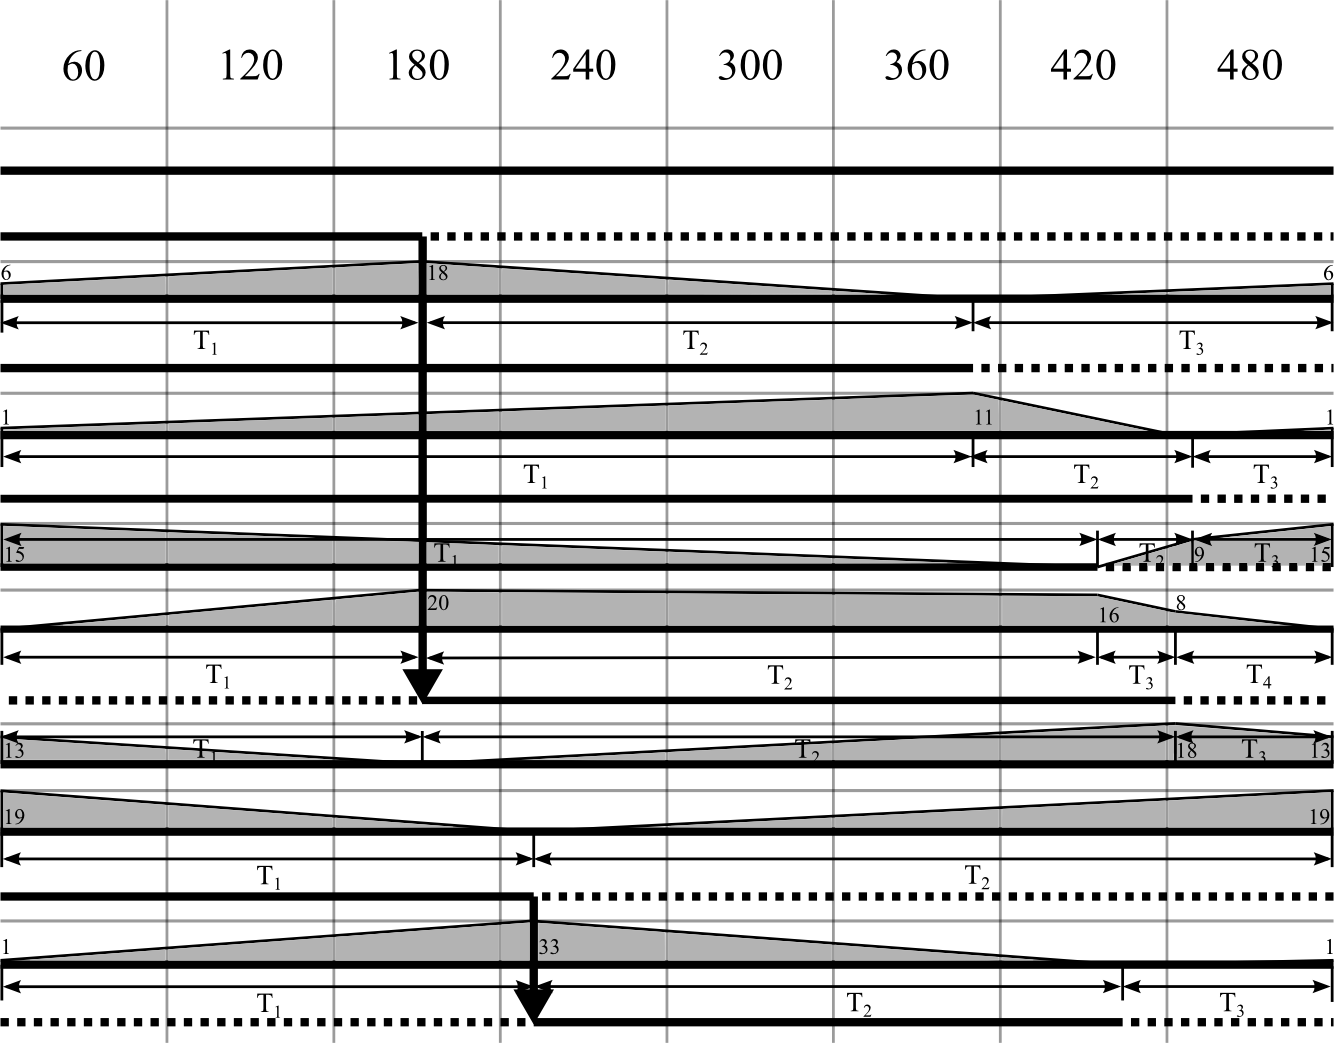
\includegraphics[width=10.7cm]{pic/splan}
       }
     }
   & \\ \cline{1-10}\cline{19-19}

   \multirow{2}{*}{1. Фрезерная} 
   & \multirow{2}{*}{5{,}82} & \multirow{2}{*}{4{,}42}
   & \multirow{2}{*}{1{,}32} & \multirow{2}{*}{2}
   & 1 
   & 100 & 480
   & \multirow{2}{*}{2}
   & 1
   & & & & & & & &
   & 83 \\

   & & & 
   & 
   & 2 
   & 32 & 152
   & 
   & 2 + v
   & & & & & & & &
   & 26 \\ \cline{1-10}\cline{19-19}

   \multirow{2}{*}{2. Шлифовальная} 
   & \multirow{2}{*}{7{,}45} & \multirow{2}{*}{4{,}42}
   & \multirow{2}{*}{1{,}69} & \multirow{2}{*}{2}
   & 3 
   & 100 & 480
   & \multirow{2}{*}{2}
   & 3
   & & & & & & & &
   & 64 \\

   & & & 
   & 
   & 4 
   & 69 & 330
   & 
   & 4 + v
   & & & & & & & &
   & 44 \\ \cline{1-10}\cline{19-19}

   \multirow{2}{*}{3. Слесарная} 
   & \multirow{2}{*}{8{,}36} & \multirow{2}{*}{4{,}42}
   & \multirow{2}{*}{1{,}89} & \multirow{2}{*}{2}
   & 5 
   & 100 & 480
   & \multirow{2}{*}{2}
   & 5
   & & & & & & & &
   & 57 \\

   & & & 
   & 
   & 6 
   & 89 & 429
   & 
   & 6 + v
   & & & & & & & &
   & 51 \\ \cline{1-10}\cline{19-19}

   4. Токарная
   & 3{,}64 & 4{,}42
   & 0{,}82 & 1
   & 7 
   & 82 & 395
   & 1
   & 7
   & & & & & & & &
   & 109 \\ \cline{1-10}\cline{19-19}

   \multirow{2}{*}{5. Фрезерная} 
   & \multirow{2}{*}{6{,}91} & \multirow{2}{*}{4{,}42}
   & \multirow{2}{*}{1{,}56} & \multirow{2}{*}{2}
   & 8 
   & 100 & 480
   & \multirow{2}{*}{2}
   & 8
   & & & & & & & &
   & 69 \\

   & & & 
   & 
   & 9 
   & 56 & 271
   & 
   & 9 + v
   & & & & & & & &
   & 39 \\ \cline{1-10}\cline{19-19}

   6. Слесарная
   & 4{,}42 & 4{,}42
   & 1{,}0 & 1
   & 10 
   & 100 & 480
   & 1
   & 10
   & & & & & & & &
   & 109 \\ \cline{1-10}\cline{19-19}

   \multirow{2}{*}{7. Сверлильная} 
   & \multirow{2}{*}{6{,}18} & \multirow{2}{*}{4{,}42}
   & \multirow{2}{*}{1{,}4} & \multirow{2}{*}{2}
   & 11 
   & 100 & 480
   & \multirow{2}{*}{2}
   & 11
   & & & & & & & &
   & 78 \\

   & & & 
   & 
   & 12 
   & 40 & 192
   & 
   & 12 + v
   & & & & & & & &
   & 31 \\ \cline{1-10}\cline{19-19}

   \multirow{2}{*}{8. Токарная} 
   & \multirow{2}{*}{6{,}36} & \multirow{2}{*}{4{,}42}
   & \multirow{2}{*}{1{,}44} & \multirow{2}{*}{2}
   & 13 
   & 100 & 480
   & \multirow{2}{*}{2}
   & 13
   & & & & & & & &
   & 75 \\

   & & & 
   & 
   & 14
   & 44 & 212
   & 
   & 14 + v
   & & & & & & & &
   & 33 \\ \cline{1-10}\cline{19-19}

   Итого
   & 49{,}27 & 4{,}42
   & 11{,}13 & 14
   & 14 
   & 79 & 
   & 12
   & 
   & & & & & & & &
   & \\ \hline

    \end{tabular}
  }
\end{table}


\end{landscape}
% \restoregeometry
   % Стандарт-план работы участка
\renewcommand{\thefigure}{\Asbuk{section}.\arabic{figure}}
\renewcommand{\thetable}{\Asbuk{section}.\arabic{table}}
\renewcommand{\thelstlisting}{\Asbuk{section}.\arabic{lstlisting}}

% \newgeometry{left=1cm,right=1cm,top=1cm,bottom=1cm}
\begin{landscape}
\section*{%
  ПРИЛОЖЕНИЕ Б \\ 
  (обязательное) \\ 
  Планировка участка (к подразделу~3.1)
}
\addcontentsline{toc}{section}{%
  Приложение Б (обязательное) Планировка участка
}
\label{sec:appendix_b}

\pagestyle{fancy}
\fancyhf{}  % clear all header and footer fields
\fancyfoot[R]{\thepage}
\renewcommand{\headrulewidth}{0pt}
\renewcommand{\footrulewidth}{0pt}

\setlength{\headheight}{10mm}
\setlength{\headsep}{\baselineskip}
\chead{Продолжение приложения \Asbuk{section}}

\thispagestyle{plain}

\setcounter{section}{1}
\setcounter{figure}{0}
\setcounter{table}{0}
\setcounter{lstlisting}{0}

\begin{figure}[h!]
  \centering
  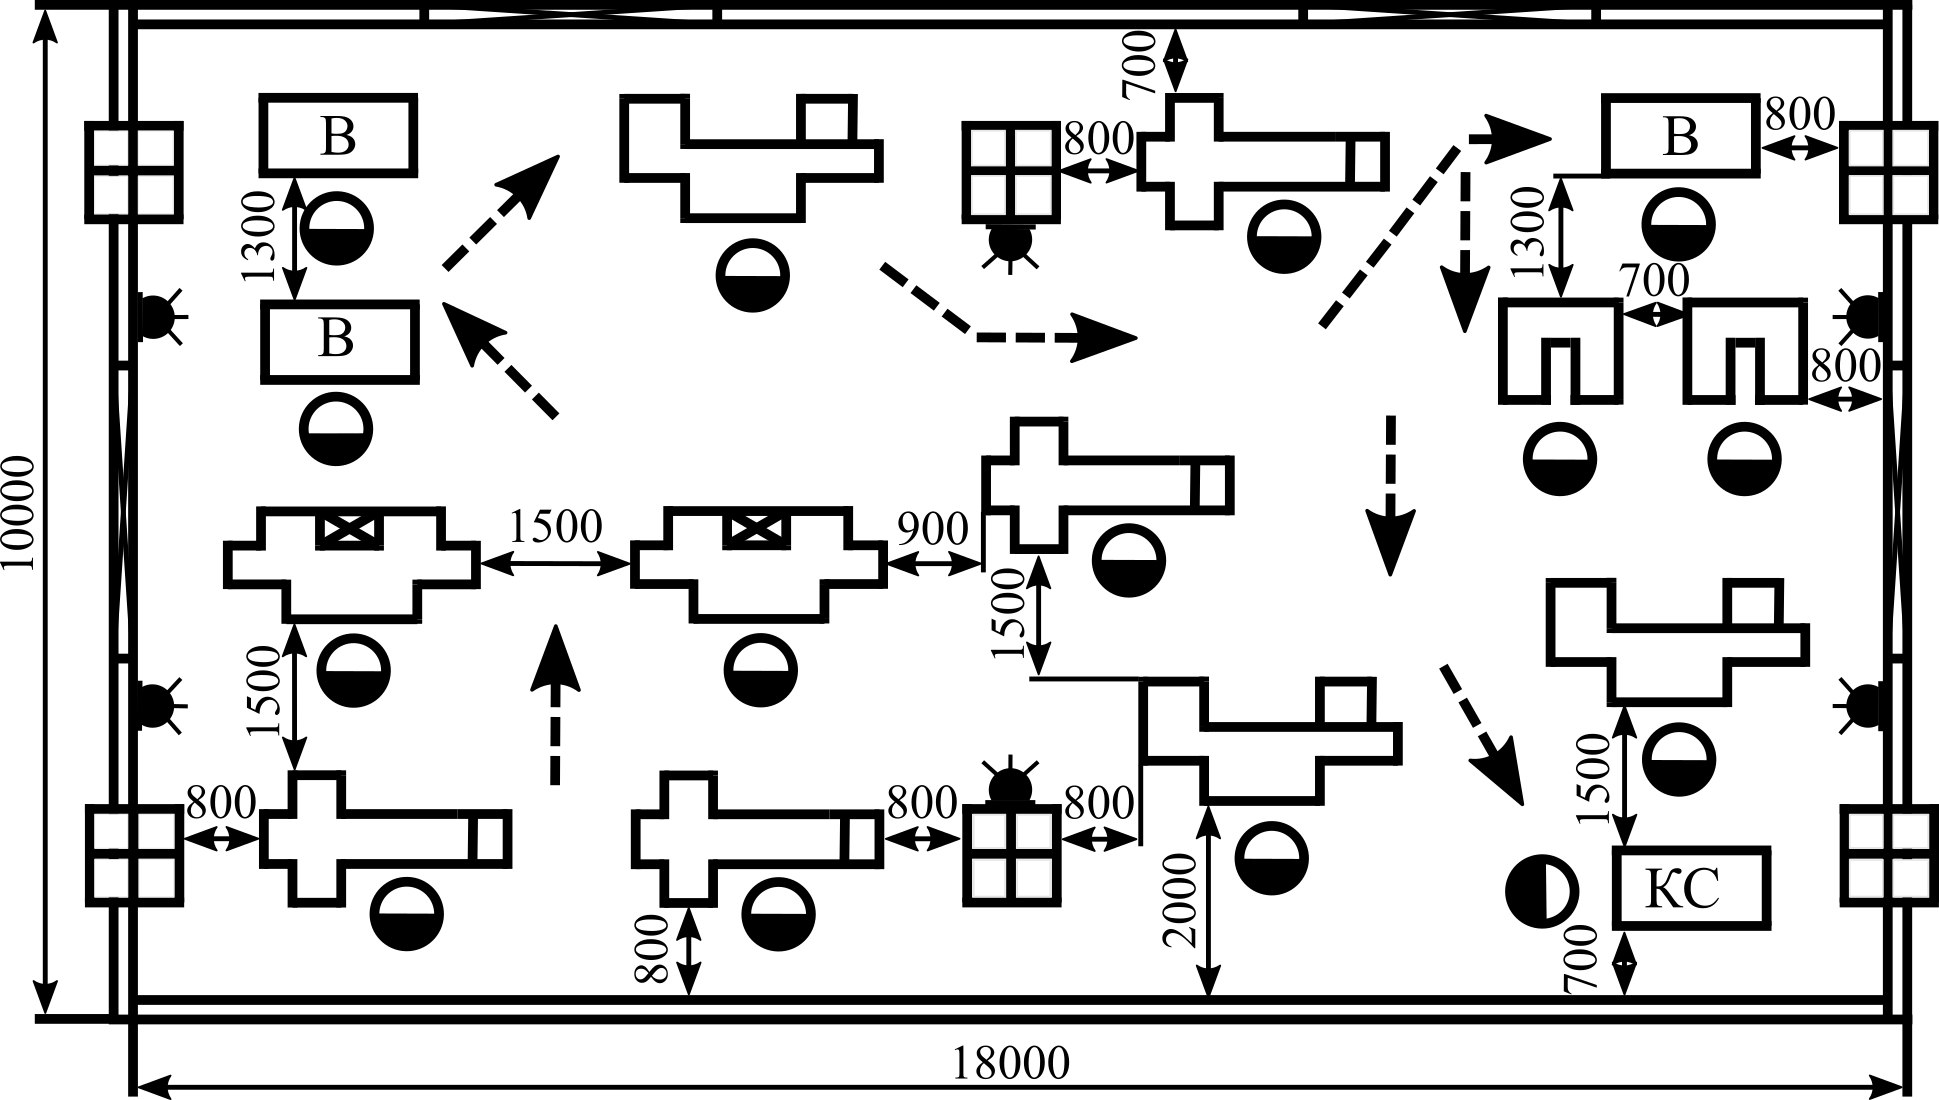
\includegraphics[width=180mm]{pic/plan.png}
\end{figure}



\end{landscape}
% \restoregeometry
   % Приложение Б

\end{document}